\documentclass[a4paper,fleqn,usenatbib]{mnras}
%\usepackage{newtxtext,newtxmath}
\usepackage[T1]{fontenc}
\usepackage{ae,aecompl}
\usepackage{graphicx}	% Including figure files
\usepackage{amsmath}	% Advanced maths commands
\usepackage{amssymb}	% Extra maths symbols
\usepackage{hyperref}

\def\grs{{GRS\,1739-278\,}}
\def\swiftx{{\em Swift-XRT\,}}
\def\swiftb{{\em Swift-BAT\,}}
\def\xmm{{\em XMM-Newton\,}}
\def\nustar{{\em NuSTAR\,}}
\def\integral{{\em INTEGRAL\,}}
\def\maxi{{\em MAXI\,}}


\def\ferg{erg~cm$^{-2}$~s$^{-1}$}
\def\arcsec{''}
\def\degr{$^\circ$}
\def\arcmin{'}
\def\iaucirc{{IAU~Circ.}}

\title[Study of low-frequency QPO in \grs]{Study of low-frequency quasi-periodic oscillations in \grs during 2014 outburst}

%\author[I. A. Mereminskiy et al.]{
%Ilya A. Mereminskiy,$^{1}$\thanks{E-mail: i.a.mereminskiy@gmail.com}
%Andrey N. Semena,$^{1}$
%Sergey Bykov,$^{1,2}$
%Ekaterina V. Filippova$^{1}$
%\\
% List of institutions
%$^{1}$Space Research Institute, Russian Academy of Sciences, Profsoyuznaya 84/32, 117997 Moscow, Russia\\
%$^{2}$MGTU, Moscow, Russia\\
%}

\author[Authors]{
Authors$^{1}$
\\
% List of institutions
$^{1}$Space Research Institute, Russian Academy of Sciences, Profsoyuznaya 84/32, 117997 Moscow, Russia\\
%$^{2}$MGTU, Moscow, Russia\\
}


\date{Accepted XXX. Received YYY; in original form ZZZ}

\pubyear{2017}

\begin{document}
\label{firstpage}
\pagerange{\pageref{firstpage}--\pageref{lastpage}}
\maketitle

\begin{abstract}
\end{abstract}
We detected low-frequency quasi-periodic oscillations (QPOs) at 0.3..2 Hz in \nustar and \swiftx observations of black hole candidate \grs during its 2014 outburst.

\begin{keywords}
X-rays: individual (\grs)  -- accretion, accretion disks	
\end{keywords}


\section{Introduction}
\label{sec:intro} 
The study of rapid X-ray variability is important, indeed.

\section{GRS 1739-278}

\grs is a typical X-ray nova, discovered during outburst in 1996  \citep{paul96} by SIGMA \citep{paul91} telescope onboard GRANAT space observatory.
Using {\it ROSAT} observation \cite{greiner96} inferred distance of 6--8.5~kpc, indicating that source may belong to Galactic bulge. 	

%\grs was discovered in 1996 by SIGMA telescope onboard GRANAT space observatory  \citep{paul96}.  
%Later GRANAT continued observations of this source \citep{vargas97} along with other X-ray telescopes: ROSAT \citep{greiner96}, RXTE and TTM/Kvant \citep{borozdin98}. The optical counterpart was found in observations carried out by ESO telescopes \citep{marti97}. . During the outburst \grs demonstrated typical behavior of the black hole candidate \citep[BHC, see e.g.][]{grebenev93, grebenev97, tanaka96, remillard06, belloni10}. The lightcurve could be described with a FRED-like (fast rise, exponential decay) shape, at the beginning of the outburst the source was in a typical low/hard state, with spectrum dominated by a power-law component with exponential cutoff at high ($\ge$100 keV) energies followed by a high/soft state with a strong blackbody component \citep{borozdin98}. Observations at VLA \citep{hjellming96} revealed presence of variable radio emission, which could be caused by jets.  \cite{borozdin00} found QPO at 5 Hz in RXTE observations conducted while the source was in the very high/soft state.

%The onset of 2014 outburst was detected by \swiftb \citep{krimm14_atel} along with \integral \citep{filippova14}. 

%At the beginning of the September, 2016 there was another, third, outburst, that 

\begin{figure*}
\centerline{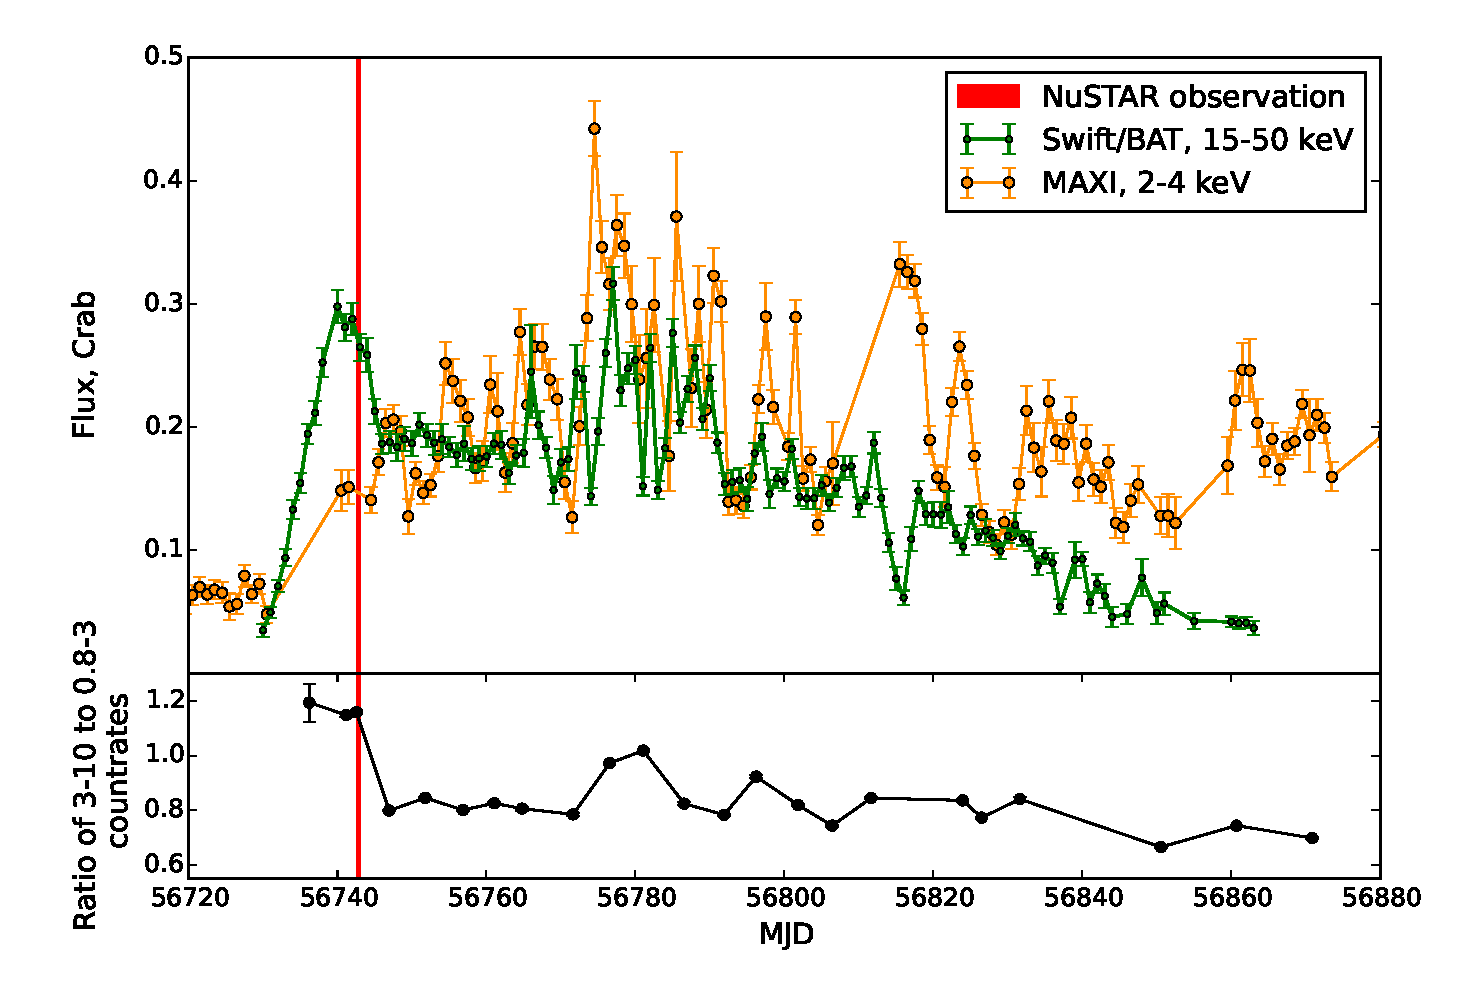
\includegraphics[scale=0.5]{batlc_v06.eps}}
\caption{{\it Upper:} green points denote \swiftb\, lightcurve of second outburst in 15--50 keV range, orange circles correspond to \maxi\, fluxes in 2--4 keV. Red line show time of \nustar\, observation. {\it Lower:} evolution of \swiftx\, spectral hardness during the outburst.} 
\label{fig:batlc}
\end{figure*} 

\section{Observations and data reduction}
\label{sec:datared} 
In order to characterize the overall outburst profile we used data of \swiftb\, {\it transient monitor} \citep{krimm13bat} in hard X-rays (15--50 keV) as well as data from \maxi\, \citep{matsuoka13maxi} (2--4 keV).

We used public observations of \swiftx\, (target ID: 33203) performed regular over the peak and decline of the outburst.  Since the source was bright, all \swiftx\, observations were performed in windowed mode, allowing study of timing properties of the source. We performed standard analysis with {\texttt{xrtpipeline}} and barycentered data prior to lightcurve extraction. 
Long-term lightcurves were obtained from UK Swift Science Data Centre at the University of Leicester \citep{evans09}.

We also used \nustar\, observation (ObsID: 80002018002) performed at March 26, 2014 (MJD 56742).  {\texttt{Nuproducts}} pipeline were utilized to extract photons  from two-arcminute circular region, centered on source and to produce lightcurves and spectra.

\section{Analysis}
\subsection{Outburst}
First detection of the source by \swiftb\, \citep{krimm14_atel} occurred at March 9, 2014 (MJD 56725, we will refer to this date as $\tau_{0}$), onset of outburst was the confirmed by \integral\, \citep{filippova14}. Outburst profile in hard X-rays (15--50~keV) featured fast rise with tenfold intensity increase over ten days, nearly flat-top peak ($\tau_{0}$+10..+15) followed by abrupt flux decrease by 30\% over two days. After this, source demonstrated gradual decline interrupted by flaring activity at $\tau_{0}$+30..+65. Another interesting feature is dip, observed in \swiftb\, lightcurve at $\tau_{0} \approx 86$. After the cease of the outburst source remained active with flux about 5--15 mCrab. 

Adding softer data from \maxi\, to the \swiftb\, hard X-ray lightcurve gives us another insight on evolution of the outburst as shown in Fig.\,\ref{fig:batlc} - comparing fluxes in soft and hard bands (for 2--4 keV band we took a 1.67 counts s$^{-1}$ as a reference value for Crab, corresponding value for 15--50 keV band is 0.22 cts cm$^{-2}$ s$^{-1}$) one can see that soft component obviously lags hard emission in the beginning of the outburst but then start to grow and ends up dominating during the flaring period as well as hard dip(s). Lower subplot of Fig.\,\ref{fig:batlc} shows evolution of hardness ratio (3--10~keV/0.8--3~keV) measured by \swiftx. Right after peak of hard X-rays one can see decline of hardness, also indicating appearance of thermal component.

This type of behavior is typical for black hole candidates \citep[BHC, see e.g.][]{grebenev97, tanaka96, remillard06, belloni10} - outburst starts from low-hard state (LHS) moves through hard intermediate state (HIMS), then proceeds to the high-soft (HSS) (or even very-high-soft state, as were seen in 1996 outburst \citep{borozdin00}) and then returns back to LHS and, eventually, to quiescence.

Fortunately, the \nustar\, \citep{harrison13_nust} observation triggered by \cite{miller15_nust} were carried right at the transition between hard and soft states, thus giving us unique possibility to study processes that happens during HIMS. 

\subsection{NuSTAR observation}
\label{sec:nust} 

\nustar\, observed \grs (ObsID: 80002018002) for nearly 30 ks of dead-time corrected exposure right after hard X-ray peak (see Fig.~\ref{fig:batlc}). Earlier, \cite{miller15_nust} shown that the average spectrum of this observation is well described by reflection models such as {\it relxill} \citep{garcia14, dauser14,dauser16} with accretion disk that reaches remarkably close to the black hole innermost stable circular orbit (ISCO), with upper estimate being $r_{in} = 5^{+3}_{-4}\, G M/c^{2}$ \citep{miller15_nust}. Interestingly, no additional thermal component was needed in order to obtain a good fit, probably because of \nustar\, energy band, starting at 3~keV. 

Given the 96.9 minute orbital period of \nustar, observation is divided in 13 intervals separated by Earth occultations, as shown in Fig.\,\ref{fig:nust_lc}. We denoted this intervals with roman numerals, from {\bf I} to {\bf XIII}. From the lightcurve of observation it is clear, that source flux is increasing throughout observation from $\approx$145 counts per second up to $\approx$170 counts per second. 
The spectrum also alter, with hardness (defined as ratio of countrates  $R_{3-10\,keV}/R_{10-78\,keV}$) monotonically growing from 2.5 to 3.5. 
Since it is obvious that the source spectrum is somehow changing during the observation it is interesting to check if Fe-line profile stays the same during observation or changes. 
We split observation into three major pieces, with first made by intervals {\bf I-IV}, second by {\bf V-IX} and third by {\bf X-XIII} and extracted 3--78 keV spectra. 
We chose to group them in order to have at least 100 counts per bin. 
Then we fitted them using \texttt{XSPEC} package \citep{arnaud96} (excluding data below 4 keV and between 5--10 keV) with simple \texttt{phabs*cutoffpl} model, using $N_{H} = 2.15\times10^{22}$ cm$^{-2}$ as was found by joint \xmm/\nustar\, observation during low luminosity state \citep{fuerst16}. Element abundances were taken from \cite{wilms00} and cross-sections from \cite{verner96}. Now, plotting the ratio of this fit to initial spectra (see Fig.~\ref{fig:ratios}) one can see that both strong features - i.e. Fe-line complex at 5--9 keV and Compton hump around 30 keV are seemingly stable. 

\begin{figure*}
\centerline{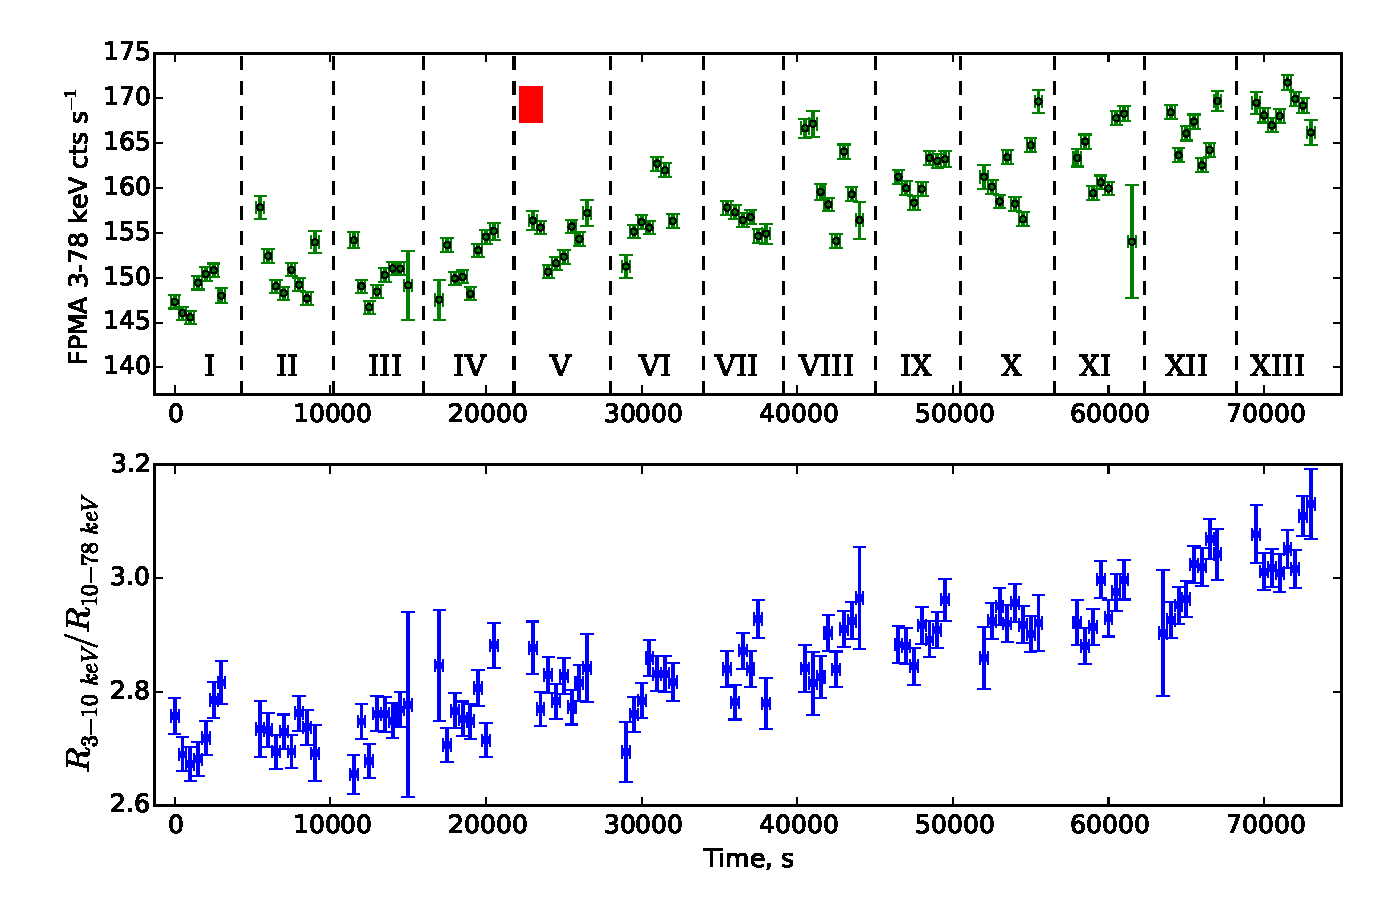
\includegraphics[scale=0.7]{nuAlc_color_v04.eps}}
\caption{Upper panel: countrate of \nustar\,FPMA in 3--78 keV band. We enumerated intervals of uninterrupted observations with roman numerals. Red square shows time of simultaneous \swiftx observation (ObsId: 00033203003, second part). Bottom panel: evolution of hardness during observation} 
\label{fig:nust_lc}
\end{figure*} 
 \begin{figure}
\centerline{\includegraphics[width=\linewidth]{ratios_v01.pdf}}
\caption{Ratio of \nustar\, spectra to \texttt{phabs*cutoffpl} model. In black - data from intervals I-IV, in red from V-IX and in blue from X-XIII.} 
\label{fig:ratios}
\end{figure}  

To get better view on evolution of continuum emission we fitted all individual interval spectra with \texttt{xillver} model \citep{garcia13}. This model describes reflection of incident radiation from ionized slab of matter. The spectrum of incident radiation are assumed to be power-law with exponential cutoff. Spectra from two \nustar\, modules from each interval were fitted simultaneously with \texttt{phabs*const*xillver} model. We choose to fix interstellar absorption at $N_{H} = 2.15\times10^{22}$ cm$^{-2}$. Relative iron abundance were fixed at
 $A_{Fe} = 1$, ionization parameter at $\xi=3.2$ and inclination at 35 degrees. This parameters are in agreement with measured by \cite{miller15_nust} with different spectral models. Although in  \texttt{xillver} there is no relativistic broadening of Fe-line no significant residuals in 5--8 keV region are seen, mainly because of limited statistics in per interval spectra. Before fitting, spectra were grouped in order to have at least 100 counts per bin, channels above 60 keV were ignored. Resulting fits are of satisfactory quality with mean $\chi^{2}_{red.} \approx 1.05$. 
 
Examination of best-fit parameters shown in Fig.\ref{fig:intspe} confirms that spectrum softens during observation and cut-off energy decreases. Flux is steadily increasing and at the end of observation unabsorbed luminosity in 3--60 keV band reach  $7\times10^{37}$ erg s$^{-1}$ assuming 8 kpc distance.

\begin{figure}
\centerline{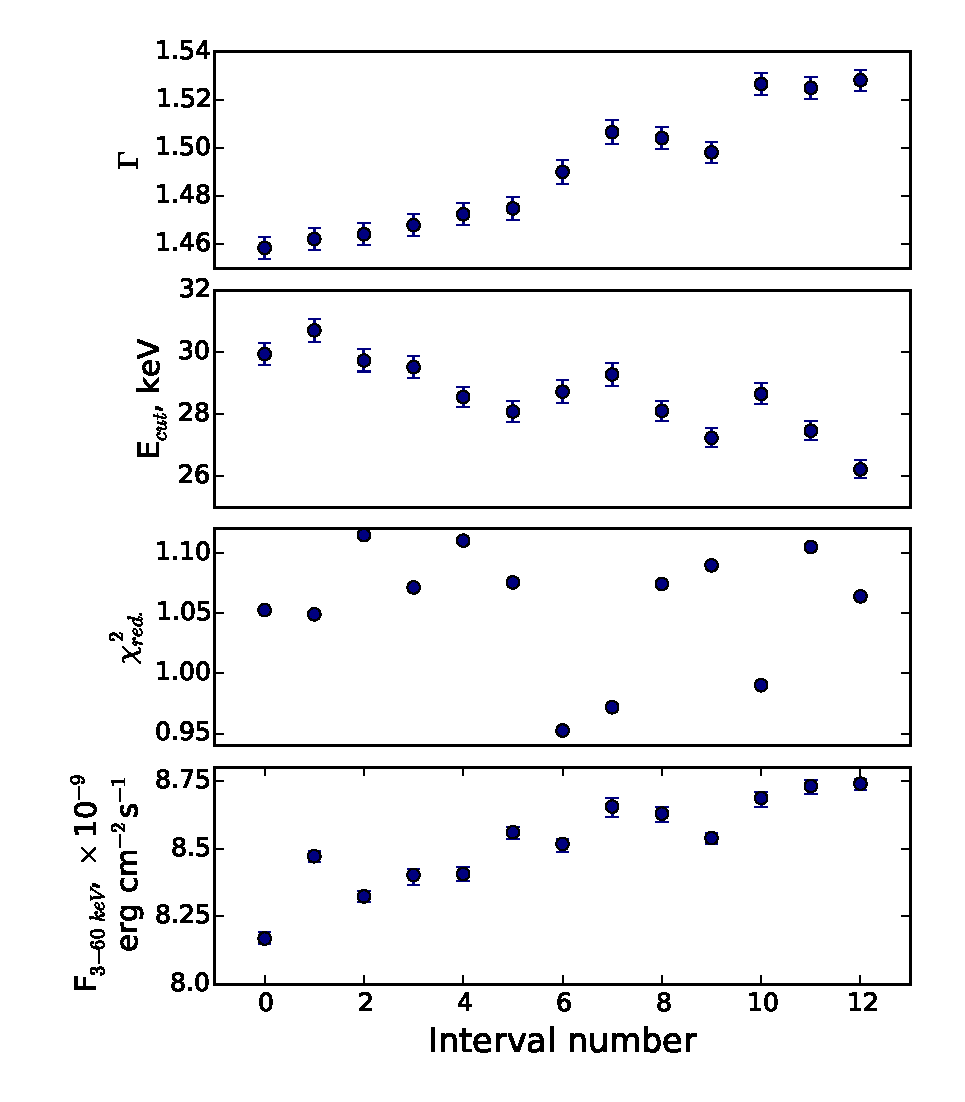
\includegraphics[width=\linewidth]{intspe_v01.eps}}
\caption{Parameters of continuum emission in intervals. } 
\label{fig:intspe}
\end{figure}  
            
There is a 1 ks part of \swiftx\, snapshot (ObsId: 00033203003) that coincides with \nustar\, observation.  Extending energy range to 0.8 to 78 keV allow one to search for thermal emission associated with cold inner disk with $kT \sim 0.1...0.4$ keV (such as were found in other BHCs during LHS, see \cite[][ e.t.c]{miller06b,miller06a,parker15}).
We used latest availiable version of {\it relxill} package (v1.0.2). 

%\begin{figure*}
%\centerline{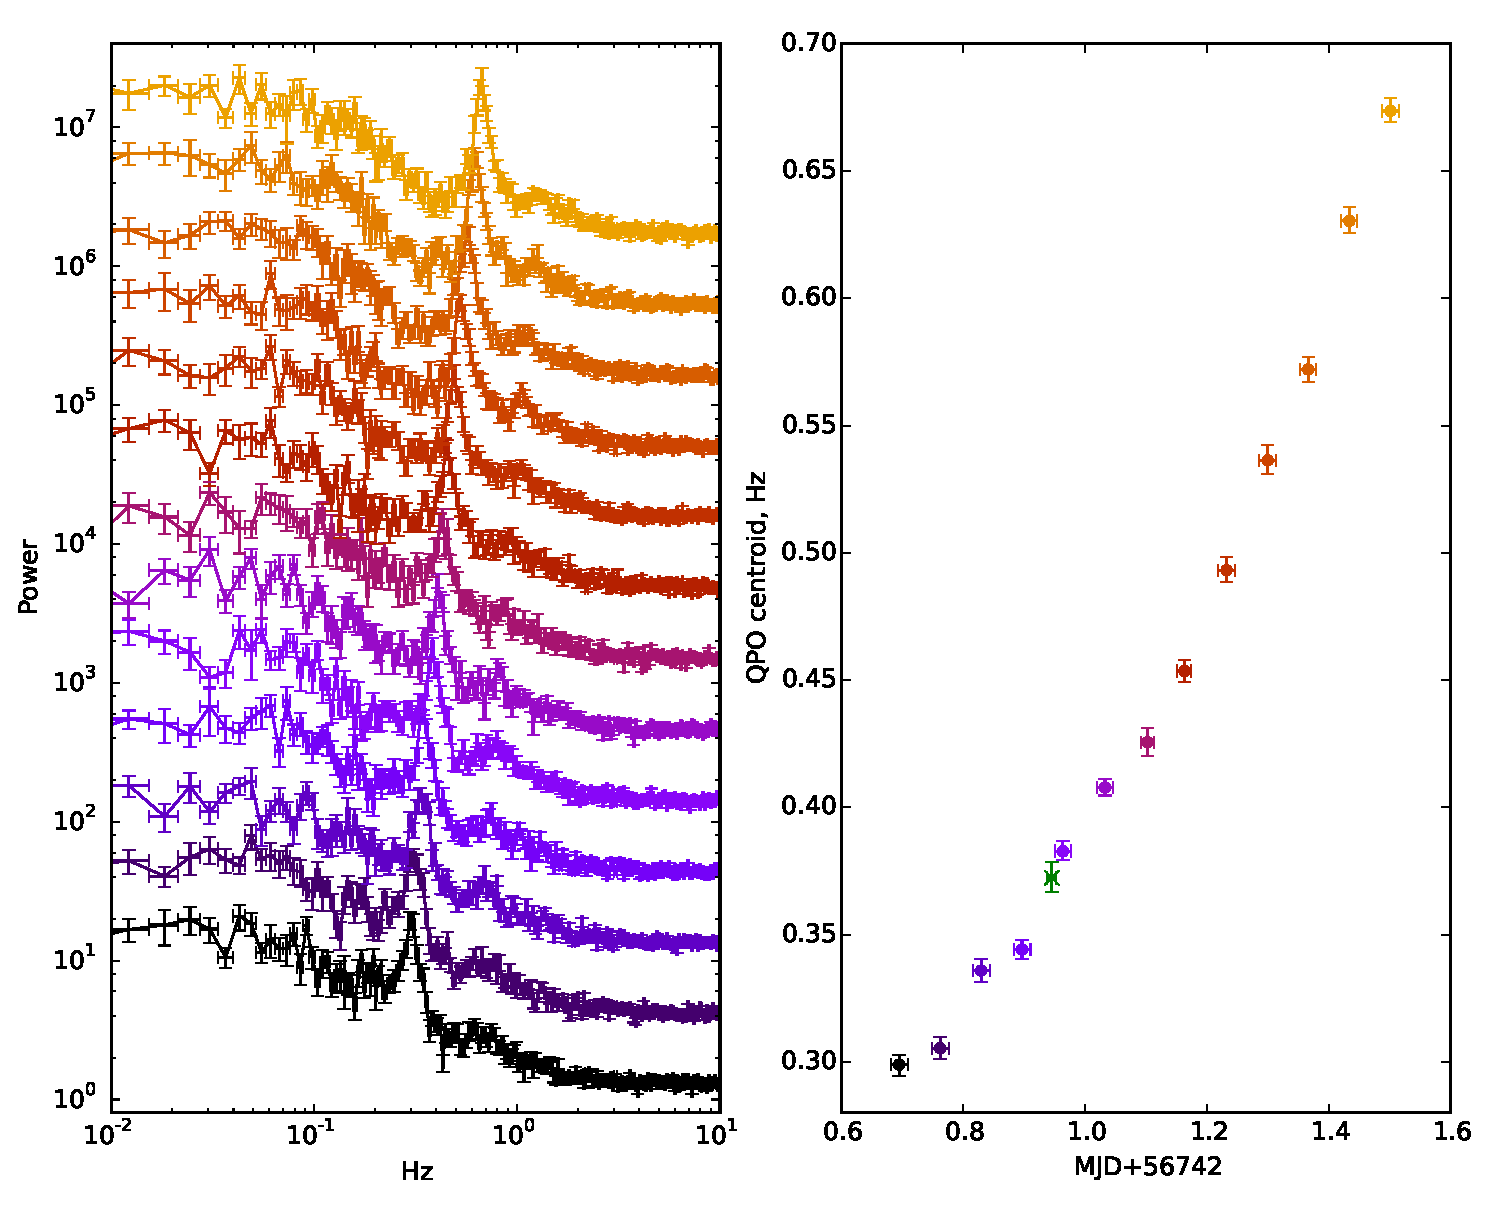
\includegraphics[scale=0.7]{QPOdrift_v02.eps}}
%\caption{Change of the QPO frequency with time. On the left panel we show how power-density spectra change with time - for clarity each spectrum is multiplied by a factor of 3.25. On the right panel we show how the QPO frequency changes during observation. Green cross show QPO frequency derived from \swiftx\, observation.} 
%\label{fig:qpodrift}
%\end{figure*}  


\section{Timing analysis} 

During recent years it was found that a lot of information about an X-ray binary could be obtained with its luminosity timing properties.
Very first one could examine luminosity variability power spectrum, which typically can be represented with the set of broad and thin Lorentzian functions representing correspondingly Fourier continuum and QPOs \citep[see, e.g.][]{1972ApJ...174L..35T, 1990A&A...227L..33B}.
It was found that variability properties changes with the system state - e.g. variability amplitude significantly lower in the soft state \citep{},  and also with the luminosity in particular state - for example position of some QPOs and the power spectrum break frequencies \cite{1990A&A...227L..33B}. 
Some aspects of the evolution of the XBs power spectrum with the system state can be explained in the frame of the accretion flow model with the geometrically thin cold disk and geometrically thick hot flow (corona), particularly it is widely accepted that the high amplitude variability is associated with the geometrically thick flow, while the geometrically thin disk is generally stable \citep{churazov}. 
It should be noted that this model of the variability generation are directly connected with the models, explaining energy spectra of black hole binaries \citep[see, e.g.,][]{1975ApJ...199L.153E, 1976ApJ...204..187S, 1995ApJ...452..710N}, \citet{churazov} has shown with the frequency resolved spectroscopy that variable part of the emission has a hard spectrum, which is thought to be produced in the corona, while stable part of the emission has a spectrum which is consistent with the cold classical $\alpha$-disc spectrum \citep{ss73}.

To explain the shape of the power spectra of the XBs different models were suggested. 
It is generally accepted that the broadband noise is produced in the coronal flow due to the stochastic variations of the angular momentum transport efficiency, \citep{lyubarskii97} model of the propagating fluctuations explains the shape of the luminosity variability power spectrum arising due to this process. 
There also a number of models, explaining high and low frequency QPO features in power spectra \citep[][]{ingram09, citesomething}. 
Most of that models were architect in order to explain energy spectra (or particular feature in it) and the power spectra. 
However, as will be discussed in the following chapter, additional analysis, describing time properties in different energy bands, can be applied to rule out some of that models.

\begin{table*}
\noindent
\centering
\caption{Evolution of the Fourier and energy spectrum properties through the {\it NuSTAR} observation}
\label{tab:timing}
\centering
\begin{tabular}{|c|c|c|c|c|c|c|c|c|c|}
\hline\hline
Data set & f$_{\rm br}$, Hz & f$_{\rm qpo}$, Hz & Q$_{\rm m}$ & Q$_{\rm o}$ & A$_{\rm m}$, (rms/mean) $\%$ & A$_{\rm o}$ (rms/mean) $\%$, rms $\%$ & \Gamma & E$_{\rm cut}$\\
\hline

I      & $7.34\times10^{-2}$   & $0.30$ & $1.04\times10^{-4}$ & $0.20$ & $0.12$ & $4.01\times10^{-2}$ & & & \\
 II     & $6.59\times10^{-2}$   & $0.31$ & $2.75\times10^{-4}$ & $0.38$ & $0.13$ & $4.76\times10^{-2}$ & & & \\
 III    & $0.11$                & $0.34$ & $7.88\times10^{-3}$ & $1.41$ & $0.12$ & $0.13$ & & & \\
 IV     & $7.08\times10^{-2}$   & $0.35$ & $2.39\times10^{-4}$ & $0.22$ & $0.13$ & $5.78\times10^{-2}$ & & & \\
 V      & $6.53\times10^{-2}$   & $0.39$ & $3.76\times10^{-4}$ & $0.53$ & $0.12$ & $4.73\times10^{-2}$ & & & \\
 VI     & $6.59\times10^{-2}$   & $0.41$ & $4.00\times10^{-5}$ & $0.10$ & $0.12$ & $3.51\times10^{-2}$ & & & \\
 VII    & $8.06\times10^{-2}$   & $0.42$ & $1.23\times10^{-4}$ & $0.16$ & $0.13$ & $4.93\times10^{-2}$ & & & \\
 VIII   & $4.03\times10^{-2}$   & $0.46$ & $2.32\times10^{-5}$ & $0.07$ & $0.13$ & $3.27\times10^{-2}$ & & & \\
 IX     & $9.01\times10^{-2}$   & $0.50$ & $2.51\times10^{-3}$ & $1.06$ & $0.13$ & $8.63\times10^{-2}$ & & & \\
 X      & $0.10$                & $0.53$ & $4.42\times10^{-3}$ & $1.02$ & $0.15$ & $0.12$ & & & \\
 XI     & $0.11$                & $0.57$ & $1.70\times10^{-3}$ & $0.99$ & $0.15$ & $7.34\times10^{-2}$ & & & \\
 XII    & $0.14$                & $0.63$ & $1.80\times10^{-3}$ & $0.82$ & $0.17$ & $8.29\times10^{-2}$ & & & \\
 XIII   & $0.13$                & $0.67$ & $1.25\times10^{-4}$ & $0.21$ & $0.15$ & $4.29\times10^{-2}$ & & & \\
\hline
\end{tabular}
\end{table*}
\subsection{Power spectrum}
    The power spectra of each of the separate observation has a form of plateau ending on the frequency $\approx0.1$~Hz transforming in the power law with the slope $\rho\approx-2$ on the higher frequencies, it also contains a prominent QPO on the frequencies 0.3--0.7~Hz and second overtone, also there is clear Poisson noise component dominating over the source variability above $\sim2$~Hz.
    The shapes of the power spectra obtained from the light curves in different energy bands are very similar.
    In order to estimate QPO amplitude and location we fit Power Spectra with the following function:
\begin{equation}
        \begin{split}
        P(f) = n (1 + (f/f_{\rm lb})^4)^{\alpha} (1 + (f/f_{\rm hb})^4)^{\beta} + \\
        \frac{s_1}{(f - f_{qpo})^2 + (f_{\rm qpo} Q_{\rm m})^2} +\\
        \frac{s_2}{(f - 2f_{qpo})^2 + (f_{\rm qpo} Q_{\rm o})^2} + \\
        n_2 (1 + (f/f_{\rm vh})^2)^{\gamma} + poiss
\end{split}
        \label{eq:complex_fit}
\end{equation}
In this function first component represents plateau function with break, which can has complex shape (sharp or wide), second two components describe QPO main harmonics and its overtone, fourth component represents any additional high frequency power, it can be connected either with the detector dead time effects or can describe broad featureless component connected to the QPO power spreading to the high frequencies, last component represents constant Poisson noise component.

\begin{figure*}
        \includegraphics[trim=0 0 0 0.65cm, clip, width=\columnwidth]{NuFirst.pdf}
        \includegraphics[width=\columnwidth, height = 0.83\columnwidth]{NuLast.pdf}
        \caption{On the left panel power spectra obtained in the soft (red) and hard (black) bands at the beginning of {\it NuSTAR} observation. 
        On the right column same spectra obtained at the end of the observation.}
        \label{fig:ps_example}
\end{figure*}

In Table \ref{tbl:ps_fit_parameters} one can fined obtained fit parameters for the 13 separate uninterrupted {\it NuSTAR} time series.

\subsection{Coherence}

    Power spectra of XBs are often have a complex shape with broad band noise and QPO like features, and numerous different models of these system were suggested to explain each particular feature. 
\citep{vaughan97} suggested to use coherence between different energy bands in order to obtain additional information on the source time properties. 
They define coherence as 
\begin{equation}
    C(f) = \frac{|<H(f)^*S(f)>|^2}{<|H(f)|^2><|S(f)|^2>}
    \label{eq:nowak_coh}
\end{equation}
where $H(f)$ and $S(f)$ are Fourier function of time series in hard and soft bands correspondingly. 
This function demonstrates the similarity of stochastic time signal in both bands. 
Different models of the XBs variability formation suggest that the signal in two energy bands can be partially independent, while the shape of the power spectra is conserved.
It appears that in many sources coherence between soft and hard X-ray bands is close to unity \citep{nowak99, wijnands01, eijden17}, in contrary to different models predictions \citep[see, discussion in][]{vaughan97}.

Following method \citep{nowak99} we estimated correlation of \grs\ light-curves obtained in the soft and hard energy bands. 
Since for the timing analysis we use {\it NuSTAR} data, we adopt following energy bands for the soft and hard light-curves correspondingly: 3--10~keV (soft) and 10--79~keV (hard).

In contrast to the \citep{nowak99} study, net count rate, obtained in \grs\ {\it NuSTAR} observation is {\bf 160~s$^{-1}$}, it follows that approximately quarter of the total variability power is due to the Poisson noise. 
As was discussed in \citep{nowak99} the correlation of two independent time series demonstrates large errors on the frequencies dominated with Poisson noise, due to the random walk in the 2-D complex space.
We also found, that the correlation of the light-curves obtained from {\it NuSTAR} is subjected by the dead-time and crosstalk effects between the energy bands.
In order to eliminate this effects, following the recipe suggested in \cite{2015ApJ...800..109B} for power spectra estimation, we find crossproducts of the light-curves Fourier functions obtained on the different modules - e.g. correlations of the light-curve obtained in the soft band on the FPMA module with the light-curve in the hard band obtained in the FPMB and vice versa.
Obtained correlation does not contain polluting signal from the blocking dead time. 

After that, as explained in \citep{Nowak99}, one should find the amplitude of the fully coherent signal $<|H(f)|^2><|S(f)|^2>$ in order to estimate coherence of the signals. 
There is several different options, which one can be use to estimate this normalization:
\begin{itemize}
        \item Use observed of the power spectra in each energy band. 
                The drawback of this method is that power spectra contain Poisson noise component constant on all frequencies and dominating over the source variability on high frequencies. 
                Thus, since Poisson noise is not coherent,  if one use this normalization as a denominator in Eq.~\ref{eq:nowak_coh} coherence estimation will be dumped on the value equal to the ratio of the Poisson noise to the source signal power on each frequency.
        \item Instead of the observed power spectra, one can use approximation of the power spectra with analytical models. 
                Poisson noise component can be discarded in analytical model, thus only source signal is conserved. 
                The drawback is that due to the Dead time effects Poisson noise has a complex form and can not be easily estimated with simple model.
        \item Use coherent part of the Fourier function of light curves in two modules \citep{2015ApJ...800..109B} or it's approximation with the analytical function. 
                It should be noted, that obtained coherent part of the ${\rm re}(H_{\rm A}(f)^*H_{\rm B}(f))$ has complex statistic which not restricting negative values, which must be ignored or modified thus affecting result.  
                We also found, that for short time series, one should use more complex likelihood criterion in order to fit coherent signal with analytical functions, since the statistic is still far from Gaussian and obtained fits are often unstable.
\end{itemize}

\begin{figure}
    \includegraphics[width=\columnwidth]{coherence_grs.pdf}
    \caption{Coherence between the soft (3--10~keV) and hard (10--78~keV) energy bands as a function of frequency} 
    \label{fig:coherence}
\end{figure}


On Figure~\ref{fig:coherence} presented measured coherence between hard and soft band on the frequencies up to $\sim1$~Hz. 
The coherence was obtained with the third method with negative values discarded. 
%This method allows to rid out of the complex high frequency features connected with the cross-talk in the energy bands and blocking dead time effects.

%There is a drawback with this method, 
%Since Poisson noise in the two considered energy bands is independent, correlation of the light-curves computed with the eq.4 from \cite{Nowak99} is dumped, and tends to zero on the frequencies where Poisson noise dominates over the source variability.
%Therefore, to obtain proper estimates on the correlation function and phase lags between soft and hard flux, instead of the product of estimates of power spectra in two energy bands as denominator we are use analytical model $P_{h}(f)\cdotP_{s}(f)$ describing corresponding power spectra. 
%Here $P_h(f)$ and $P_s(f)$ - analytical function, approximating the power spectra in soft and hard bands.
%We found, that the power spectra in this bands are very similar to each other and can be fitted on the frequencies above 0.01~Hz with the following function:


%We found, that our estimate on the coherence, growths significantly on the frequencies above $\sim2$~Hz, where Poisson noise begins to dominate over the source intrinsic variability.
%This can be explained with the uncertainty of the obtained model parameters or its simplicity. 
%We found that for both soft and hard bands, obtained fits suggest very abrupt drop in power between the QPO and low-frequency plateau, it leads to very steep index of the power-law component. 
%Therefore growth of the coherence estimates on the higher frequencies is due to the underestimation of the source intrinsic variability on the corresponding frequencies.

%We found, that, similarly to different XBs, light curves in the hard and soft bands demonstrate strong correlation up to the high frequencies, however, we were not able to estimate properly coherence above 2~Hz due to the Poisson noise.

\subsection{Phase lags}
    Most of the models of the accretion flow which describe variability and energy spectra formation, suggest the time lag between the signals in different energy bands. 
For example in some models of the energy spectra formation, time lag is naturally arise due to the geometry of the corona and properties of the inverse Comptonization process \citep[see, e.g.][]{kotov01}.
Phase lag is also suggested from the propagating fluctuations model - hard photons are emitted from the inner parts of the accretion flow from the perturbations, which initially were born in the outer parts of the disk were produce soft emission.  

It also was found, that phase lag of XBs, probably depends on the system inclination angle \citep{eijeden17}, it also definitely contain information about the characteristic times of the system, and therefore can be proxy to the compact object mass \citep{}. 

Phase lags can be estimated as a product of the mean phase of the set of Fourier spectra and the corresponding frequency:
\begin{equation}
        \begin{split}
                \tau = \frac{<\phi(f)>}{\pi f}\\
                <\phi(f)> = <arccos{\left(\frac{re(F_h(f)F_s(f))}{|F_{\rm h}(f) F_{\rm s}(f)|}\right)}>
        \end{split}
\end{equation}
here, $F_h(f)$ and $F_s(f)$ are Fourier functions of the light-curves in the hard and soft bands, $\phi(f)$ is the phase lag. 

Due to the significant fraction of the Poisson noise in each observation we were not able to obtain phase lag for them.
In order to improve significance we compute phase lag for all 13 time series.
Obtained phase lag for frequencies from $10^{-3}$~Hz to 10~Hz is presented in Figure~\ref{fig:phase_lag}.

\begin{figure}
        \includegraphics[]{}
        \caption{Phase lag between hard (10--78~keV) and soft (3--10) energy bands in \grs\ source.}
        \label{fig:phase_lag}
\end{figure}

\subsection{timinig discussion}
We found that the total power in the second QPO harmonic in the soft band is comparable to the total power in the main harmonic, in the hard band second harmonic is $\approx3$ times less powerfull than the main. 
Total power of the harmonics growing with the source count-rate and QPO frequency in the soft and hard energy bands (see Table~\ref{tab:timing}). 
If the QPO has geometrical origin - i.e. it's due to the change of the view on the some statical illumination pattern like in the \citep{IVK09} model, than this pattern is more complex in the soft energy band. 

%If the QPO is due to the changing of our field of view on some static pattern, like in the \citep{ivk09} model, than it follows that QPOs in this bands have different origin - i.e. QPO in the soft band is due to the scattering of the photones from precessing corona, while QPOs  reflection of the ro

\section*{Acknowledgments}

%--------------------------------------------------------------------------------
\bibliographystyle{astron}
\bibliography{author_en.bib,coherence.bib}
\bsp	
\label{lastpage}
\end{document}
